\section{REORDERING}
The second method to decrease memory required to solve the transport of
photons-electrons involves reordering the energy groups to simplify the
scattering cross-section matrix. When CEPXS generates the cross sections,
it first writes all the cross sections for one particle type, and then, the cross
sections for the other particle type into the scattering matrix. The
energy range is the same for the two particles. The cross section matrix looks like :
\begin{equation}
\Sigma = 
\begin{pmatrix}
PP & EP\\
PE & EE
\end{pmatrix}
\end{equation}
where PP and EE are lower triangular matrices which represent the
scattering for each particle type. The two matrices are lower triangular
because only down scattering is allowed. The cut-off energy used in
radiotherapy approximations forbids the 
thermalization of particles. Matrix EP represents the creation of photons by
electrons through bremsstrahlung production and fluorescence production.
Matrix PE represents the creation of electrons by photons through photoelectric 
effect, Compton scattering, pair electron production, and Auger production 
following photoionization. Now it is important to notice that because 
of energy conservation, a particle can only create a particle which has a 
energy equal or lower than its own. An example of the transfer
of two photon groups and four electron groups can be seen in \hbox{Figure
\ref{joli} :}
\begin{figure}[H]
\begin{center}
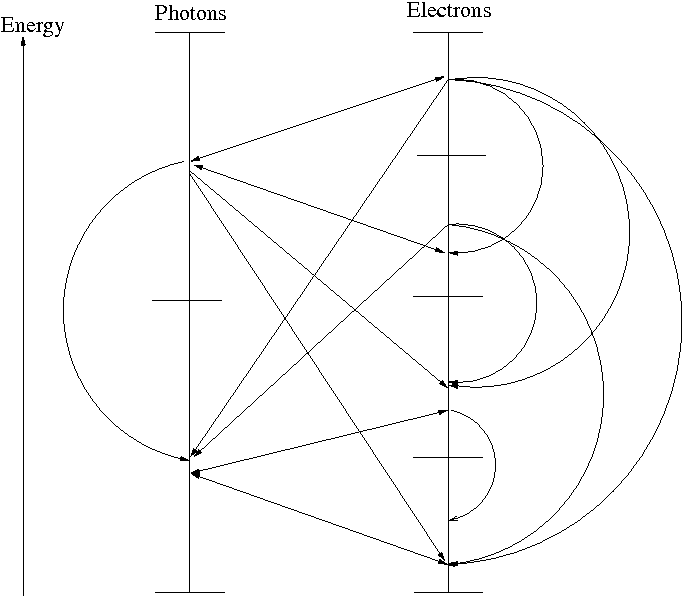
\includegraphics[height=7cm]{group.png}
\caption{\bf{Transfer between the different groups}}
\label{joli}
\end{center}
\end{figure}
The pattern of the scattering matrix is as follows :
\begin{equation}
\Sigma =
\begin{pmatrix}
x & 0 & \vline & x & x & 0 & 0\\
x & x & \vline & x & x & x & x\\
\hline     
x & 0 & \vline & x & 0 & 0 & 0\\
x & 0 & \vline & x & x & 0 & 0\\
x & x & \vline & x & x & x & 0\\
x & x & \vline & x & x & x & x\\
\end{pmatrix}
\end{equation}
We can see that there is no upscattering to the first group of photons, the
first and the second group of electrons coming from the second group of
photons, and the third or the fourth group of electrons (see Figure
\ref{joli}). If we reorder the groups using for the first group \hbox{set :} 
photon group 1, electron group 1, electron group 2 and for the second group 
\hbox{set :} photon group 2, electron group 3, electron group 4. The pattern 
of the scattering matrix looks \hbox{like :}
\begin{equation}
\Sigma =
\begin{pmatrix}
x & x & x & \vline & 0 & 0 & 0\\
x & x & 0 & \vline & 0 & 0 & 0\\
x & x & x & \vline & 0 & 0 & 0\\
\hline      
x & x & x & \vline & x & x & x\\
x & x & x & \vline & x & x & 0\\
x & x & x & \vline & x & x & x\\
\end{pmatrix}
\end{equation}
Now, we see that the matrix is block lower triangular and we can solve the
transport problem by solving two problems with only three groups each. 
We can solve the first three groups without solving the last three groups since 
there is no upscattering coming from these. Then, we can solve the last three 
groups, with the first three groups hidden in the source term. 
If there are more than two group sets, the fixed source,
which now contains the scattering source, can be saved on an auxiliary
memory, like for example on the hard disk. Only the source for the groups of the
group set that we are solving are needed in memory.
To know how many groups we need to gather from each particle 
in each group set, we can use a simple rule. First, we define the number of
photon groups as $n_p$, the number of electron groups as $n_e$ and the 
greatest common divisor between these two numbers as $gcd$. The number of
photon groups to put in a group set is $\frac{n_p}{gcd}$ and the number 
of electron groups to put in a group set is $\frac{n_e}{gcd}$. Instead 
of solving one problem of $n$ groups, we can solve $gcd$ problems of 
$\frac{n}{gcd}$ groups. Notice that we assumed that CEPXS generates groups of
equal energy per groups. This is only one of the two ways used by CEPXS to
generate the cross sections. For the other one, the energy per group varies 
logarithmically. In this case, if we assume that $n_e \geq n_p$, we will have 
$n_p$ group sets, $n_p-1$ group sets containing each one electron group and one 
photon group and one group containing the photon group of lowest energy and 
the $n_e-(n_p-1)$ electron groups of lowest energy.\\
Reordering the groups can also decrease the number of source iteration or
GMRES iterations. These two methods are used to solve the linear system 
created by the discretized transport equation of (\ref{solved}).
Below, we compare the number of iterations needed to
solve a problem similar to the one described in the previous section with and
without reordering. The domain is
made of aluminium, we use a $S_{12}$ angular discretization and $P_5$ expansion
for the scattering cross section. We use linear discontinuous finite elements 
for the spatial discretization. The range of energy studied is [0.01MeV,10MeV]. 
There are 180 cells and we have 15 groups of photon and 25 groups of electron.
We compare three methods : the standard multigroup iterative scheme, the
standard multigroup iterative scheme with reordering and the blocked
multigroup iterative scheme. The last scheme solves eight multigroup
transport problems, each of them having only five groups.
We obtain the following result :
\begin{table}[H]
\begin{center}
\caption{\bf{Comparison of the number of iterations with and without group
reordering}}
\begin{tabular}{|c|c|c|c|}
\hline
&\multicolumn{2}{c|}{With reordering} & Without reordering\\
\hline
&Modified multigroup & Standard multigroup & Standard multigroup\\
\hline
Total inner iterations & 4232 & 6956 & 7398\\ 
Total outer iterations & 17 $\approx$ 2 per block & 5 & 5\\
\hline
\end{tabular}
\end{center}
\end{table}
Reordering the groups decreases the number of inner iterations by 6\% while
the blocked scheme reduces the number of inner iterations by 42\% compare to the
standard multigroup scheme.
